\chapter{Background and Literature review}

\section{Business Process Management}

BPM has been viewed from highly diverse angles ranging from a management strategy to a software system, so much so, that there is still not a common consensus even about the definition of the name itself~\cite{van2003workflow}. BPM includes methods, techniques and tools to support the design, enactment, management and analysis of business processes~\cite{van2003workflow}.

BPM is a cycle methodology where several perspectives of BPs are investigated during its various stages~\cite{lodhi2013business}. In order to effectively understand BPM terminologies and features, we start with an overview of the BPM life cycle.

According to Van-Der-Aalst~\cite{van2003workflow}, the BPM life cycle comprises four stages: process design, system configuration, process enactment and diagnosis.
\begin{itemize}
    \item In the process design stage, the AS-IS BPs are electronically modelled into the BPMS by using graphical standards, such as UML and BPMN.
    \item In the system configuration stage, the BPMS and the underlying system infrastructure are configured. 
    \item In the process enactment stage, electronically modelled BPs are deployed in the BPMS engines. by using execution standards, such as BPEL and BPML.
    \item In the diagnosis stage, the BPM analysts define and improve bottlenecks in the BPs by using analysis and monitoring tools, such as business activity monitoring (BAM)) and process mining .
\end{itemize}

\section{Terminology}


This section presents the terminology used in this project.
It is based on the definitions by Wil van der Aalst~\cite{Aalst2013} and Marlon Dumas~\cite{dumasFundamentalsBusinessProcess2018} [REF].Different organisation use different terms for overlapping concepts. The Table~\ref{table:terminology} provide explanation about terms in this paper.

\begin{table}[htb]
\footnotesize	 %changing the font size
\begin{tabularx}{\textwidth}{X X}

\hline
Terms in this paper   & Explanation \\
\hline
Process instance~\cite{van2011process} & A \textit{process instance} represents one specific instance of a process that is currently executing \\
\hline
Process mining~\cite{Aalst2013} & \textit{Process mining} is a technique to analyze and track processes.\\
\hline
Document Number~\cite{dumasFundamentalsBusinessProcess2018} & It is the unique ID for each activities  \\
\hline
Tasks~\cite{Aalst2013} & A business process is composed of \textit{tasks}. \\
\hline
Role & Each lane represents a \textit{role} in the problems section~\pageref{figure:soAndfieldservice}  . \\
\hline
Trace & Each business process instance contains a \textit{trace} over the business process. \\
\hline
Case &  A particular \textit{case} may have more than one process instance associated with it \\ 
\hline
Case Id & Each~\textit{case} can be identified by its individual case ID and can have attributes with different values\\
\hline
activity & An action or task that can be performed for a process instance (conceptual level) \textit{process instance}\\
\hline
Event log & It is required to contain a case id ,activity description, and timestamp . \\
\hline
Resource~\cite{Aalst2013} & Process mining use extra information the \textit{resource}(i.e., person or device) executing or initiating the activity \\
\hline
Process models~\cite{dumasFundamentalsBusinessProcess2018} & The result of process discovery is generally a \textit{process model}. \\
\hline
Petri nets~\cite{Aalst2013} & One of process models. \\
\hline
Process Discovery~\cite{Aalst2013} & Visual representation of all cases of the dataset. \\
\hline
Process variant~\cite{Aalst2013} & visual representation of the most important variants of the dataset.. \\
\hline
Conformance checking~\cite{Aalst2013} & compare real process with BPMN model. \\
\hline
Cycle time~\cite{Aalst2013} & The time it takes for one process run to complete the full set of activities to accomplish a business process. \\
\hline
Event~\cite{Aalst2013} & event = case + activity + timestamp + etc. \\
\hline
Timestamp~\cite{Aalst2013} & A time indication consisting of a date and possibly a time part(instance level) \\
\hline


\end{tabularx}
\caption{current terms explanation}
\label{table:terminology}
\end{table}


To avoid confusion came from using different terminologies , the term will be used to describe the comprehensive list  combining and explaining used terms and others terms. The analysis of terminology collected from literature and summarized in Table~\ref{table:terminology}



% We follow BPMN as basis.

% \begin{itemize}
%     \item A business process is composed of \textit{tasks}.
%     \item Each lane represents a \textit{role}.
%     \item A business process instance corresponds to the execution of the business process to a particular case. 
%     \begin{itemize}
%         \item Each business process instance contains a trace over the business process (the activities that have been performed for that particular instance).
%     \end{itemize}
%     \item ...
% \end{itemize}


\section{Business Process Mining}

While BPM covers the methods, techniques and tools that support the design, management and analysis of business processes ~\cite{van2003workflow}, data mining refers to the extraction of knowledge from data produced by a set of systems and processes. The combination of BPM and data mining has generated the new field of study known as process mining ~\cite{van2011process}, which aims to apply data mining techniques to data from the BPM lifecycle ~\cite{song2008trace} to extract in-depth insights from the event logs of workflow and BPM systems ~\cite{van2003workflow}.



Figure ~\ref{figure:BPMJ} introduces the components of process mining. Initially, the majority of process mining contributions focused on techniques for the discovery of processes (business process analysis), conformance checking (business process monitoring, business activity monitoring and process performance management) and various extensions ~\cite{song2008trace}, represented by the lower part of Figure 1. To enable these techniques, researchers also focused on log file preparation and mining algorithms ~\cite{weijters2006process}. Therefore, the first series of process mining papers primarily addressed the lower part of Figure ~\ref{figure:BPMJ}. Tiwari et al. ~\cite{tiwari2008review} drew attention to the relationship between the process model and event logs by reviewing state-of-the-art process mining algorithms. Using 50 analyzed papers, they classified those that used process mining techniques and identified six practical challenges. The process mining manifesto ~\cite{van2012process} renewed these challenges and identified 11 challenges. While Tiwari et al. ~\cite{tiwari2008review} primarily addressed problematic log file preparation (e.g., noise, hidden tasks, duplicate tasks, etc.), the challenges of the process mining manifesto have a broader perspective covering the application and representation of process mining, e.g., balancing quality criteria such as fitness, simplicity, precision and generalization, cross-organizational mining and operational support.


\begin{figure}[!htb]
    \centering 
    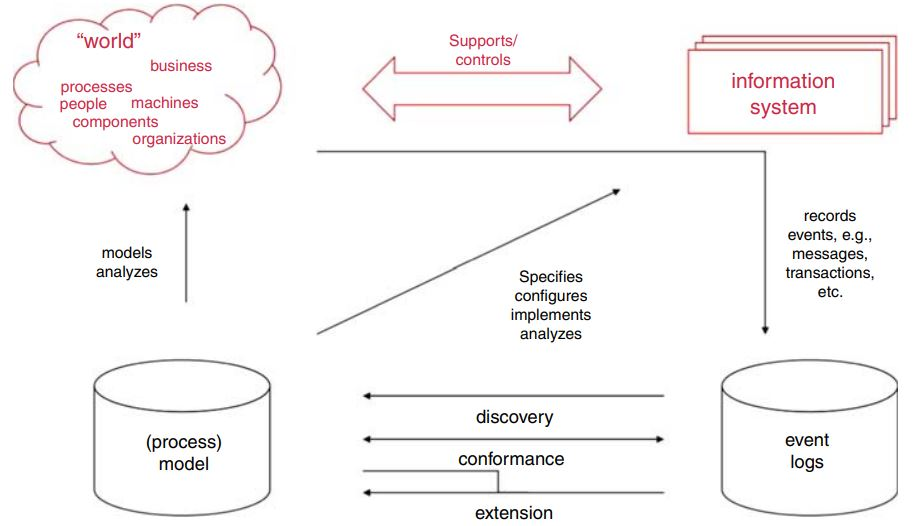
\includegraphics[scale=0.7]{resource/BPMJ.JPG}
    \caption{source: Adpoted from Van der Aalst ~\cite{van2011process}}
    \label{figure:BPMJ}
\end{figure}



The study of event logs and how they are extracted from ISs (right part of Figure 1) are addressed by Rozinat and van der~\cite{rozinat2006decision}, de Medeiros and Günther ~\cite{de2005process} and Adriansyah et al. ~\cite{adriansyah2011conformance}. In these studies, the conformance of event logs and real world or reference models is assessed. Other authors address the use of process models in real-world accounting (left part of Figure 1), e.g., for forced behavior ~\cite{wen2009novel}, concept drift ~\cite{engel2014case} and security ~\cite{van2005process}. Finally, Maruster et al. ~\cite{muarucster2006rule} discuss noise cancellation in event logs.

Later research focuses more on the upper-red part of Figure 1, i.e., the relationship between the “world” and ISs. While Turner ~\cite{turner2012process} provide an overview of the process mining tools available in the UK market, other studies address either the combination of process mining with other technologies (e.g. artificial neural networks, support vector machines) ~\cite{maita2015ultraflexible} or a specific application area (e.g. healthcare) ~\cite{rojas2016process} ~\cite{yang2014process}. Our study follows Rojas’s path and addresses the relationship between the “world,” more specifically, “organizations,” and IS, which is marked in red in Figure 1. Similar to the most recent reviews (~\cite{kurniati2016process}; ~\cite{maita2015process}; ~\cite{rojas2016process}), we follow a systematic literature review approach. However, we adopt a broader scope to analyze empirical studies on process mining that is not limited to a specific market or application area.

\section{Process Mining Tools}

Describe the tools here.

\section{Final Considerations}
